\subsubsection{Biochemistry and Cell Biology - MHC class I Trafficking}
\index{Springer, Sebastian}

\paragraph{Research Team}
%
Sebastian Springer (Professor), Ute Claus (Lab Technician), Britta Borchert (PhD Student), Malgorzata Garstka (PhD Student), Esther Ghanem  (Graduate Student), Clemens Schneeweiss (PhD Student), Praveen Pudiavettil Tayakuniyil (PhD Student), Anca Tigan (Graduate student), Rakina Yaneva  (Graduate Student)\\

We investigate the molecular mechanism of the antiviral immune response. When a mammalian cell is infected by a virus, the fragments (peptides) of its proteins are pumped into the Endoplasmic Reticulum (ER). There, they bind to receptor proteins called MHC class I molecules which then move to the cell surface. Cells that thus expose viral peptides on their surfaces can be killed by the immune system, and the spread of the virus halted.
Empty MHC class I molecules cannot go to the cell surface. In the ER, they are bound by the class I loading complex, a group of proteins. One of these proteins, tapasin, binds directly to class I molecules and helps them to quickly find peptides that make stable complexes; it is also required to keep empty class I molecules in the ER.
We investigate the folding, peptide binding, and ER export of class I molecules. Our research helps to understand protein folding and transport in general, and will suggest ways to manipulate the immune response.

\paragraph{Highlights}
This year, we have shown conclusively that peptide-free MHC class I
molecules have access to both the ER-Golgi intermediate compartment,
and the cis side of the Golgi apparatus, meaning that they cycle
between the ER and these compartments, instead of being strictly
retained in the ER. We have performed confocal fluorescence
microscopy to observe the distribution of class I molecules, but we
have also finished the work on an in vitro transport assay that
recapitulates the sorting of cargo proteins into COPII vesicles that
bud from the ER and go to the ERGIC. In these transport vesicles, we
have detected empty class I molecules, which confirms the microscopy
results. Thus, we have shown for the first time that in normal
cells, completely and incompletely folded forms of the same protein
can be exported from the ER at the same time. (Garstka, Borchert, et
al., submitted.) Intriguingly, it seems that class I molecules in
the COPII vesicles have a lower affinity to peptides - perhaps the
purpose of the cycling of class I molecules between ER and Golgi is
to bring them into different chemical environments and vary the
binding affinity of the complex in order to accelerate the binding
of high-affinity peptides. Which features of a peptide allow class I
molecules to go to the cell surface? If we electroporate peptides
into living fibroblasts, the class I molecules move to the cell
surface. This novel assay allows us to test many peptides in live
cells. Remarkably, we have found that peptides which lack the two
C-terminal amino acids cannot induce the ER exit of class I even if
they bind to class I very tightly (as established through
fluorescence spectroscopy in collaboration with Werner Nau, IUB).
\begin{figure}[ht]
  \begin{center}
   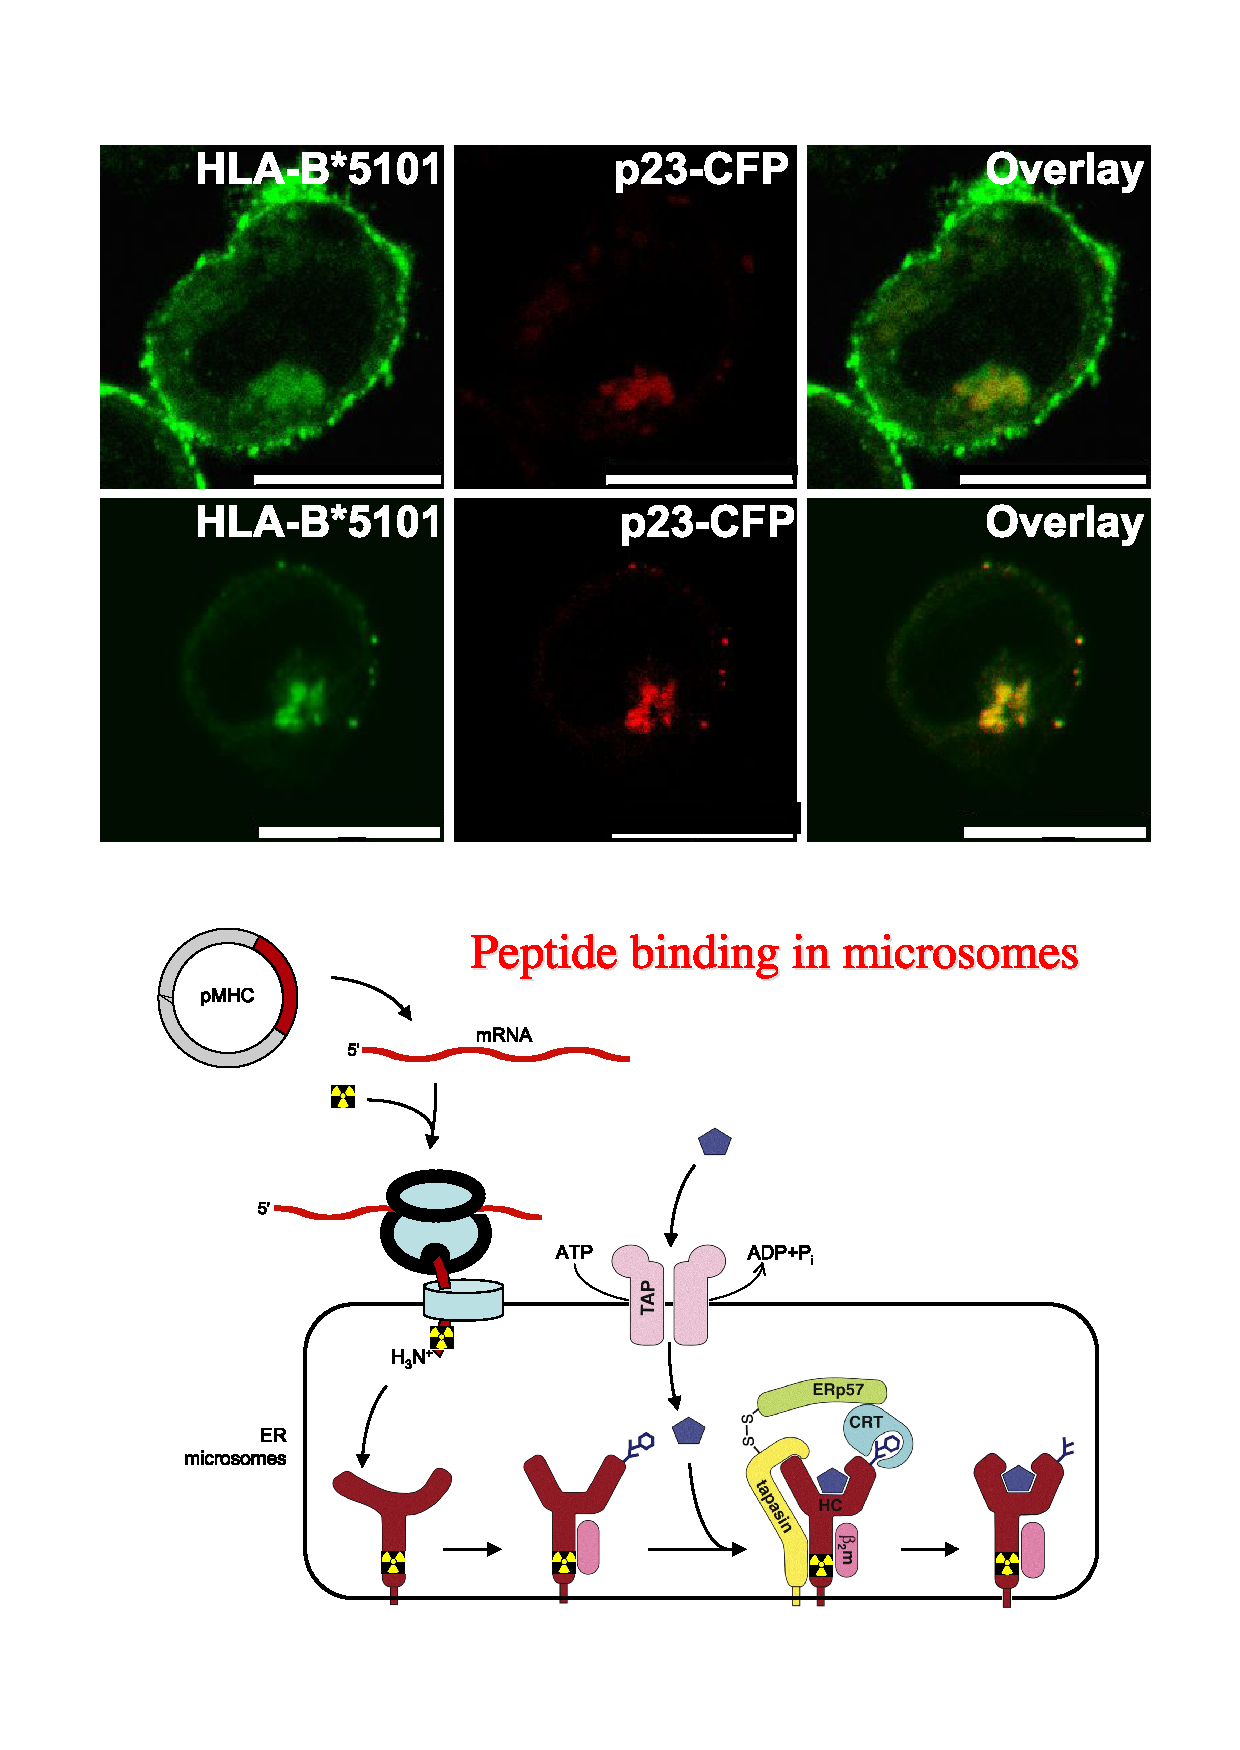
\includegraphics[width=\hsize]{Springer/Springer_2006_Fig.pdf}
    \mycaption{Upper panel, Class I molecules (HLA-B*5101) colocalize with the cis side of the Golgi apparatus (labeled through the protein, p23) in wild type (top) and mutant (bottom) cells. Lower panel, peptide binding in microsomal membranes: principle of the assay.}\label{fig:Springer}
   \end{center}
\end{figure}

This agrees with Martin Zacharias' findings that the carboxy
terminus of the peptide induces a conformational change in the class
I molecule when it binds (Zacharias and Springer, 2004). Thus, cells
scan the region of the class I molecule that binds the C terminus of
the peptide when they check for peptide occupancy. This result once
again implicates tapasin which binds to that region of class I.
Continuing our collaboration with the Zacharias group at IUB, they
have found in further molecular dynamics simulations that
tapasin-dependent class I molecules find it difficult to stay closed
without peptide while tapasin-independent class I molecules are
closed most of the time (Sieker et al., in press). To assess the
effect of tapasin on peptide binding under realistic ER conditions,
we have established an assay for peptide binding to class I in
microsomal membranes. Class I molecules are transcribed, translated
(with $^{\mbox{{\footnotesize 35}}}\mbox{S}$ radioactive label),
translocated into the microsomes, folded, and associated with the
light chain (beta-2 microglobulin) in vitro. We can then translocate
peptides into the microsomes and detect their binding to the class I
molecules. In the coming year, this assay will be done in microsomes
from mutant cells to determine the influence of individual
chaperones, including tapasin, on class I assembly and peptide
binding.




\paragraph{Organization}
%
International University Bremen Contact Person of the GBM (German
Society for Biochemistry and Molecular Biology).



\paragraph{Grants}
\begin{enumerate}
\item Funded by DFG,  \emph{ER to Golgi transport of MHC class I
molecules}, SP 583/2-2, (February 2004 - January 2007)
\end{enumerate}

\paragraph{Other Support Grants}
\begin{enumerate}
\item Two DAAD scholarships for PhD students
\item EMBO short-term traveling fellowship for a PhD student
\end{enumerate}


\myparagraph{Collaborations}
%
Bremen Area Collaborations:
\begin{enumerate}
\item {\sl International University Bremen} \\  Dr. N. K�hl \\ MHC class I and HLG expression in the brain
 \\  Prof. W. Nau \\ Fluorescence spectroscopy of recombinant MHC class I molecules.
 \\  Prof. M. Winterhalter \\ Injection of engineered nanocapsules into cells for use as sensors.
 \\  Prof. M. Zacharias \\Dynamics of tapasin-dependent and -independent class I molecules in their empty and peptide-bound form, and the mechanism of action of tapasin.

\end{enumerate}
National \& International Collaborations:
\begin{enumerate}
\item {\sl Universit�t Osnabr�ck} \\ Heinz-J�rgen Steinhoff \\ Electron paramagnetic resonance of MHC class I molecules.
\item {\sl Southampton University} \\ Tim Elliott \\ Cell biology of tapasin action on MHC class I molecules.
\item {\sl Southampton University} \\ J�rn Werner \\ NMR studies of tapasin interaction with MHC class I molecules.
\item {\sl Royal Holloway University} \\ Rainer Duden and Irina Majoul \\ Confocal laser scanning microscopy of class I molecules in live cells.
\end{enumerate}



\nocite{Springer1,Springer2,Springer3}
